\documentclass[a4paper, 10pt, twocolumn, twoside]{article}
\usepackage[margin={1.5cm}]{geometry}
\usepackage{hyperref}
\setlength{\columnsep}{0.75cm}
\usepackage{adjustbox}
\usepackage[utf8]{inputenc}
\usepackage[T1]{fontenc}

\usepackage{enumitem}
\setlist{itemsep=0pt,parsep=0pt, topsep=0pt, leftmargin=11pt}

\usepackage{multicol}
\usepackage{courier}
\renewcommand{\familydefault}{\ttdefault}
\renewcommand{\labelitemi}{-}
%\usepackage[norsk]{babel}
\usepackage[none]{hyphenat}


\usepackage{wrapfig}

\usepackage{sectsty}
\usepackage{titlesec}

\sectionfont{\underline}
\subsectionfont{\underline}
\titlespacing*{\section}{0pt}{-0em}{0pt}
\titlespacing*{\subsection}{0pt}{-0.5em}{0pt}
\titlespacing*{\subsubsection}{0pt}{0em}{0pt}

\usepackage{color}
\usepackage{xcolor}

\setlength{\parindent}{0em}
\setlength{\parskip}{1em}


\date{}
\title{Hemmelig Hitler\vspace{-3em}}

\begin{document}
\definecolor{naziorange}{HTML}{F86640}
\ttfamily
\maketitle

\begin{center}
    \textbf{Norwegian Rules for Secret Hitler}    
\end{center}
\textit{Året er 1932. Stedet er Tyskland. I Riksdagen prøver politikerne å holde liv i demokratiet. Men blant dem finnes det fascister i forkledning. Og én av dem er en Hemmelig Hitler.}
\begin{center}
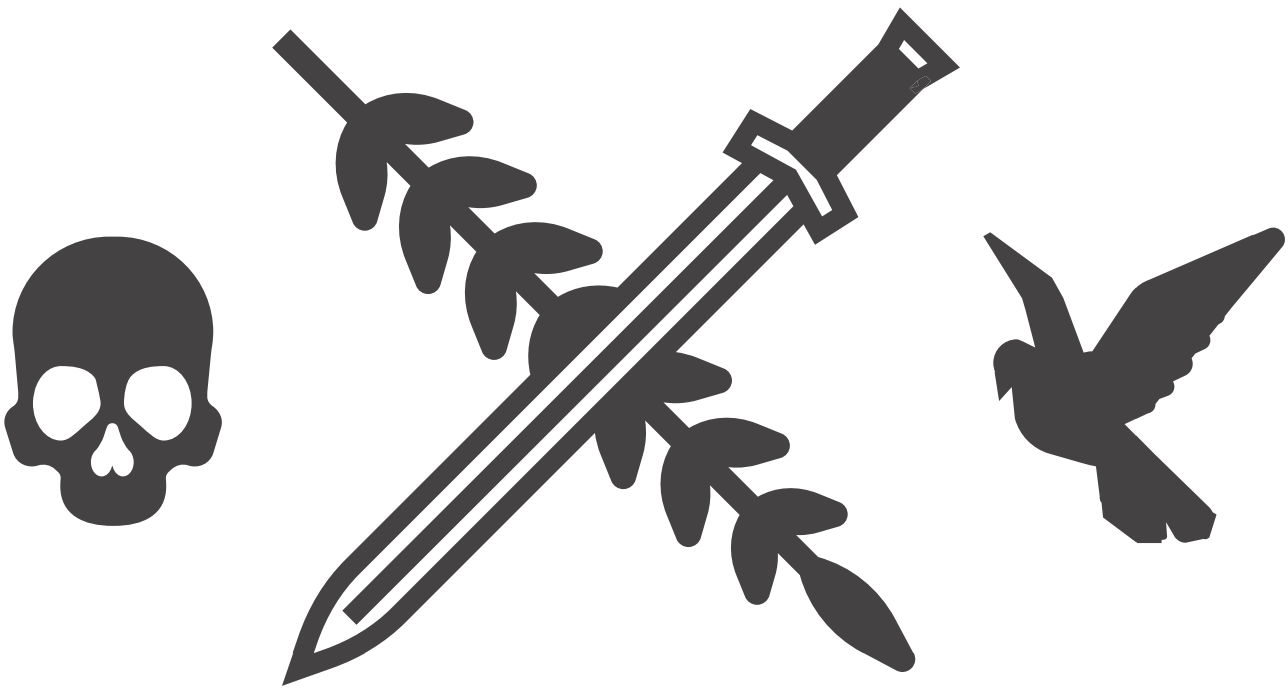
\includegraphics[width=0.7\columnwidth]{./graphics/hitler_skalle_og_due}
\end{center}


\section{I korte trekk}
Ved spillets begynnelse blir hver spiller tildelt én av tre roller: \textbf{liberal}, \textbf{fascist} eller \textbf{Hitler}. De liberale er i flertall, men vet ikke hva de andre er. Fascistene og Hitler jobber på lag mot de liberale. Fascistene kjenner hverandre og vet hvem Hitler er, men Hitler vet ikke hvem som er fascister (med unntak av når det er 5 eller 6 spillere).  

\begin{itemize}
    \item \textbf{De liberale vinner dersom fem liberale lovforslag blir innført eller Hitler henrettes.}
    \item \textbf{Fascistene vinner dersom seks fascistiske lovforslag blir innført eller Hitler blir valgt til kansler etter at tre fascistiske lovforslag er blitt innført.}
\end{itemize}

Når et fascistisk lovforslag blir innført, kan det føre til at den sittende presidenten får spesielle privilegier som må brukes før spillet kan fortsette, samme hvilket lag presidenten faktisk tilhører. Dette kan friste selv en liberal president til å innføre fascistiske lovforslag.

\section{Mål}
Alle spillere får utdelt en hemmelig identitet. Ut fra denne spiller man enten på det liberale eller det fascistiske laget.

\parbox{\columnwidth}{
De liberale vinner dersom 
\begin{itemize}
    \item fem liberale lovforslag innføres
    \item[] \textit{\uppercase{eller}}
    \item Hitler blir henrettet.
\end{itemize}
}

\parbox{\columnwidth}{
Fascistene vinner dersom
\begin{itemize}
    \item seks fascistiske lovforslag innføres
    \item[] \textit{\uppercase{eller}}
    \item Hitler blir valgt til kansler etter at tre eller flere fascistiske lovforslag er innført.
\end{itemize}
}
\section{Spillets innhold}
\begin{itemize}
\item 17 lovforslag (6 liberale, 11 fascistiske)
\item 10 rollekort
\item 10 partimedlemskapskort
\item 10 konvolutter
\item 10 ja!-kort
\item 10 nein!-kort
\item 1 valgmarkør
\item 1 trekkebunkekort
\item 1 kastebunkekort
\item 3 liberal/fascist-brett
\item 1 presidentbrikke
\item 1 kanslerbrikke
\end{itemize}

\section{Forberedelser}
Velg fascist-brett etter hvor mange det er som skal spille og legg det ved siden av liberal-brettet. Bland lovforslagskortene (11 fascistiske og 6 liberale) og legg dem i en trekkebunke med billedsiden ned. Gi alle spillerne ett \textit{ja!}- og ett \textit{nein!}-kort hver.

Finn frem så mange konvolutter som det er spillere. Hver eneste konvolutt kommer til å inneholde ett rollekort og ett partimedlemskapskort. Bruk tabellen nedenfor til å finne ut hvor mange som trengs av hver.

Dersom en konvolutt inneholder et liberalt rollekort, skal man også legge et liberalt partimedlemskapskort i den. Konvolutter med fascist- og Hitler-rollekort skal ha fascistiske partimedlemskapskort.

\begin{adjustbox}{max width=\columnwidth}
\begin{tabular}{l|c|c|c|c|c|c}
\textbf{\# Spillere} & \textbf{5} & \textbf{6} & \textbf{7} & \textbf{8} & \textbf{9} & \textbf{10} \\ \hline
Liberale          & 3          & 4          & 4          & 5          & 5          & 6           \\ \hline
Fascister         & 1+H        & 1+H        & 2+H        & 2+H        & 3+H        & 3+H         \\
\end{tabular}
\end{adjustbox}

\textit{Forsikre dere om at kortene er fordelt riktig før dere fortsetter. }

Når konvoluttene er klare, stokkes de slik at ingen vet hvilken rekkefølge de ligger i. Gi én konvolutt til hver spiller og vent med å åpne dem. Når alle har fått en konvolutt, ser hver enkelt på sine egne kort.
{\color{naziorange}
\fbox{\parbox{0.97\columnwidth}{
\setlength{\parskip}{1em}
\textbf{Hvorfor er det både rolle- og parti\-medlemskapskort?}

Senere i spillet hender det at presidenten får undersøke hvilket parti en annen spiller tilhører. Dersom en liberal president hadde fått vite at den undersøkte var Hitler, hadde det blitt altfor lett for de liberale å vinne. Derfor får man et partimedlemskapskort, slik at en slik undersøkelse ikke avslører forskjellen på Hitler og en vanlig fascist.}}
}

Velg tilfeldig hvem som skal være den første presidentkandidaten. Gi president- og kanslerbrikkene til denne spilleren.


\textbf{Når det er 5 til 6 spillere}, si følgende instrukser til alle spillere:
\textit{\begin{itemize}
\item Alle sammen, lukk øynene.
\item Fascister og Hitler, åpne øynene og se på hverandre. Hitler, gi et tegn til resten om hvem du er.
\item[] [Ta en lang pause]
\item Alle sammen, lukk øynene igjen.
\item Nå kan alle åpne øynene. Hvis noen er forvirret eller noe har gått galt, må man si det nå.
\end{itemize}}

\textbf{Når det er 7 til 10 spillere}, si følgende instrukser til alle spillere:\textit{\begin{itemize}\item Alle sammen, lukk øynene og strekk frem en lukket neve med tommelen fri.
\item Fascister, men ikke Hitler, åpne øynene og se på hverandre.
\item Hitler, hold øynene lukket og løft tommelen opp.
\item Fascister, merk dere hvem Hitler er.
\item[] [Ta en lang pause]
\item Alle sammen, lukk øynene igjen og ta ned tommelen.
\item Nå kan alle åpne øynene. Hvis noen er forvirret eller noe har gått galt, må man si det nå.
\end{itemize}}

\section{Spillets gang}
Hemmelig Hitler spilles i runder. I hver runde skal man \textbf{avholde valg}, \textbf{innføre et lovforslag} og benytte seg av eventuelle \textbf{privilegier}.

\subsection{Avholde valg}
1.\ \textbf{Send presidentbrikken mot venstre}\\
Den som mottar brikken er den nye presidentkandidaten.

2.\ \textbf{Utnevn en kanslerkandidat}\\
Presidentkandidaten sender kanslerbrikken til en valgbar spiller for å vise hvem han eller hun vil stille til valg med.

\textbf{Valgbarhet:}
Presidenten og kansleren som sist ble valgt sitter i karantene. De kan ikke utnevnes til kanslerkandidat i neste runde.

{\color{naziorange}
\fbox{\parbox{0.97\columnwidth}{
\textbf{Mer om valgbarhet:}
\begin{itemize}
\item Karantenen gjelder presidenten og kansleren som sist \textit{ble valgt}, ikke de som sist stilte til valg.
\item Karantenen hindrer deg kun i å stille som kanslerkandidat. Man kan være presidentkandidat selv om man var kansler i forrige runde.
\item Hvis det bare er fem spillere igjen i spillet, gjelder karantenen kun den forrige kansleren. Presidenten kan altså stille til kansler i neste runde.
\item Det er to ting som har en spesiell påvirkning på valgbarhet: Vetoretten og valgtelleren. Ikke bry deg med disse ennå; de blir forklart i hvert sitt avsnitt senere.
\end{itemize}
}}
}

3.\ \textbf{Stem på regjeringen}\\
Når presidentkandidaten har utnevnt en valgbar kanslerkandidat, kan spillerne diskutere den foreslåtte regjeringen frem til alle er klare til å stemme. Alle spillere, inkludert kandidatene, skal avgi stemme. Når alle har bestemt seg, rekker alle frem stemmesedlene med billedsiden ned og snur dem samtidig. På denne måten er alle stemmer lett synlige, og ingen kan ombestemme seg ut fra hva andre har stemt.

\textbf{Dersom det er uavgjort eller flertallet har stemt nei:}

Kandidatene ble ikke valgt inn. Presidentbrikken går videre til neste spiller. Valgtelleren flyttes ett felt.

\textbf{Valgtelleren:} Hvis spillerne forkaster tre foreslåtte regjeringer på rad, henfaller landet til kaos. Trekk det øverste lovforslaget fra trekkebunken og innfør det. Dersom feltet som forslaget legges på gir spesielle privilegier, får ingen utføre disse. Valgtelleren settes tilbake til start. Alle spillere kan igjen utnevnes til kanslerkandidat. Hvis det er færre enn tre lovforslag igjen i trekkebunken, stokkes disse sammen med kastebunken til en ny trekkebunke.

\textit{Når et lovforslag havner på bordet med billedsiden opp, betyr dette at valgtelleren skal tilbake til start, uavhengig av om det ble innført av en valgt regjering eller et misfornøyd folk.}

\textbf{Hvis et flertall stemmer ja:}

Kandidatene trer nå inn i rollene som president og kansler. De skal innføre et nytt lovforslag.

\textbf{NB: Hvis tre eller flere fascistiske lovforslag allerede er innført:}

\textit{Spør kansleren om han eller hun er Hitler. Hvis svaret er ja, er spillet over og fascistene har vunnet. (Hvis svaret er nei, er spilleren garantert ikke Hitler.)}

\subsection{Innføre et lovforslag}
Når president og kansler er valgt, skal de jobbe sammen om å innføre en ny lov. Presidenten trekker de tre øverste lovforslagene i trekkebunken og ser på disse i hemmelighet. Presidenten legger ett av forslagene med billedsiden ned i kastebunken og sender de to gjenværende forslagene til kansleren. Kansleren ser på dem og legger ett av dem, også dette med billedsiden ned, i kastebunken. Til slutt legger presidenten det gjenværende lovforslaget med billedsiden opp på det tilsvarende brettet på bordet. 

All kommunikasjon, muntlig eller ikke, mellom president og kansler er forbudt mens dette pågår. Det er også viktig at presidenten og kansleren med viten og vilje velger hvilke forslag som skal som kastes, sendes videre og innføres. De har altså ikke lov til å spille ut tilfeldige lovforslag, for eksempel ved å stokke forslagene og velge tilfeldig. Presidenten må alltid sende begge lovforslag videre til kansleren samtidig; hen kan ikke sende dem enkeltvis for å se på kanslerens reaksjon. Hemmelig kommunikasjon, tilfeldighet og andre forstyrrelser mens man innfører lover er et angrep på spillets ånd. Hev dere over slikt.

\textbf{Forkastede lovforslag skal \textit{aldri} vises til resten av spillerne. Spillerne må ta presidenten og kansleren på deres ord. Presidenten og kansleren står fritt til å lyve.
}

{\color{naziorange}

\fbox{\parbox{0.97\columnwidth}{
\textbf{Angående løgn}: Ofte får noen spillere vite ting som resten ikke vet, som når regjeringen får se lovforslag eller når presidenten får undersøke en annen spillers partitilhørighet. Man kan alltid lyve om slik skjult kunnskap i Hemmelig Hitler. Det eneste tilfellet der man er nødt til å snakke sant er når man kan avslutte spillet. Hitler må altså si ifra dersom han eller hun blir henrettet og dersom han eller hun blir valgt til kansler når tre eller flere fascistiske lovforslag er innført.
}}
}

\textbf{Hvis det er færre enn tre lovforslag igjen i trekkebunken når en lov er blitt innført}, skal disse stokkes sammen med kortene i kastebunken og bli en ny trekkebunke. Ubrukte lovforslag skal aldri vises frem, og de \textit{må} stokkes inn. De skal altså \textit{ikke} legges til side og plasseres øverst i den nye trekkebunken.

\textbf{Hvis regjeringen vedtok et fascistisk lovforslag som havnet på et felt med et privilegium}, må den sittende presidenten benytte seg av dette. 

\textbf{Hvis regjeringen vedtok et lovforslag som havnet på et blankt felt}, begynner man en ny runde.

\subsection{Spesielle privilegier}
Dersom et fascistisk lovforslag innføres og det medfører et spesielt privilegium, må presidenten benytte seg av dette før neste runde kan begynne. Før presidenten benytter seg av det, kan han eller hun diskutere saken med resten av spillerne, men når alt kommer til alt er det presidenten som har siste ord på når og hvordan makten skal brukes. Spillet kan ikke fortsette før presidenten har benyttet seg av privilegiet. Privilegiene blir brukt opp; de gjentas altså ikke når senere forslag blir innført. Et privilegium spares heller ikke til senere dersom en lov blir innført som følge av at valgtelleren når toppen. 

\subsubsection{Presidentens privilegier}

\textbf{Undersøke tilhørighet}\\
\begin{wrapfigure}{r}{0.2\columnwidth}

\includegraphics[width=\linewidth]{./graphics/hitler_glass}
\end{wrapfigure}
Presidenten velger seg en spiller å undersøke. Den undersøkte sender partimedlemskaps\-kortet (ikke rollekortet!)\ til presidenten, som undersøker kortet uten å vise det til andre. Presidenten kan fortelle (eller lyve om) hva som sto på kortet. Ingen spiller kan undersøkes to ganger i løpet av samme spill.

\textbf{Skrive ut særvalg}\\
\begin{wrapfigure}{r}{0.2\columnwidth}

\includegraphics[width=\linewidth]{./graphics/hitler_hatt}
\end{wrapfigure}
Presidenten utnevner en hvilken som helst annen spiller til å være neste presidentkandidat ved å sende presidentbrikken til denne. Hvem som helst kan bli presidentkandidat, også en kansler i karantene. Den nye presidenten utnevner en valgbar kanslerkandidat, og valget avholdes som vanlig.

\textbf{Et særvalg fører ikke til at rekkefølgen forskyves på noen måte etter denne runden. Etter at valget er avholdt, med eventuelle lover og privilegier som konsekvens, går presidentbrikken tilbake til den som egentlig skulle ha vært neste presidentkandidat før særvalget ble skrevet ut.}

Dersom presidenten sender presidentbrikken videre til neste spiller i rekkefølgen (spilleren til venstre) vil denne få være presidentkandidat to ganger på rad:\ én gang i særvalget, og enda en gang når man går tilbake til normalen.

\textbf{Titte i trekkebunken}\\
\begin{wrapfigure}{r}{0.2\columnwidth}

\includegraphics[width=\linewidth]{./graphics/hitler_bunke}
\end{wrapfigure}
Presidenten ser på de tre øverste lovforslagene i trekkebunken og legger dem tilbake uten å vise dem til andre eller endre rekkefølgen.

\textbf{Henrettelse}\\
\begin{wrapfigure}{r}{0.2\columnwidth}

\includegraphics[width=\linewidth]{./graphics/hitler_kniv}
\end{wrapfigure}
Presidenten henretter en spiller ved bordet ved å si «Jeg henretter offisielt [henrettedes navn]». Dersom den henrettede er Hitler, betyr dette at de liberale har vunnet. Hvis den henrettede ikke er Hitler, får spillerne ikke vite noe om den henrettede, uansett tilhørighet. Henrettede spillere er døde, og kan naturlig nok ikke snakke, stemme eller stille til valg.

\subsubsection{Vetorett}
Vetoretten er en spesialregel som trer i kraft når fem fascistiske lovforslag er innført. Fra da av kan en valgt regjering la være å innføre en lov dersom kansleren foreslår det og presidenten er enig. 

Som vanlig trekker presidenten tre lovforslag, kaster ett og sender de to gjenværende videre til kansleren. Kansleren kan nå si «Jeg ønsker å legge ned veto mot disse forslagene». Dersom presidenten svarer «Jeg er enig», legges begge forslagene i kastebunken og presidentbrikken blir sendt videre mot venstre. Hvis presidenten ikke er enig, må kansleren innføre et av dem, som vanlig. 

Når regjeringen benytter vetoretten, er dette et tegn på handlingslammelse. Misnøyen blant folket øker, og valgtelleren flyttes derfor ett felt frem.

\section{Strategi}
\begin{itemize}
    \item \textbf{Enhver spiller bør hevde å være liberal}. Siden de liberale er i flertall, vil de raskt kunne straffe enhver som hevder å være fascist. Derfor gir det ingen fordeler for en fascist å avsløre sin tilhørighet. De liberale bør alltid snakke sant, ettersom de samarbeider om å løse samme gåte. Alle løgner gjør denne gåten vanskeligere for dem.
    \item \textbf{Hvis dette er første gang du har rollen som Hitler, husk å spille så liberalt som mulig.} Vedta liberale lovforslag. Stem på liberale regjeringer. Kyss spedbarn. Stol på at undersåttene dine gir deg liberale lovforslag og at de selv tar hånd om å fremme fascismens sak når du er utenfor mistanke. Som fascist vinner man ved å manipulere de liberale og å ha en god løgn i bakhånd når man må spille fascistisk – ikke ved å gå åpent ut som skurk.
    \item \textbf{Liberale drar som regel fordel av å spille sakte og å diskutere det som har skjedd.} Fascister drar som regel fordel av å spille raskt og å skape forvirring.
    \item \textbf{Fascister vinner som regel ved å få Hitler valgt til kansler, ikke ved å innføre seks fascistiske lovforslag.} Å velge Hitler som kansler er kjernen i en vellykket fascistisk strategi. Hitler burde alltid spille liberalt og unngå krangler, løgner og mistanke – for når tiden er inne, trenger Hitler de liberales tillit for å bli valgt. Og selv om man ikke lykkes med å få Hitler valgt til kansler, er tvil blant de liberale nøkkelen til å få fascister i maktposisjoner sent i spillet.
    \item \textbf{Spør andre spillere om hvorfor de gjorde som de gjorde.} Dette er spesielt viktig når presidenten får privilegier. Faktisk kan det være lurt å spørre presidentkandidater om hvem de kunne tenke seg å undersøke, utnevne eller henrette hvis de fikk sjansen.
    \item \textbf{Hvis et fascistisk lovforslag havner på bordet, finnes det tre mistenkte: presidenten, kansleren og/eller trekkebunken.} Prøv å finne ut hvilke av dem som har skylden.
\end{itemize}

\section{Takk}
Mike, Tommy, Max og Mac ønsker å takke:

Shari Spiro, Ginny Miller, Dan Shapiro, Elan Lee, Mike Selinker, Luke Crane og alle andre hos Kickstarter, alle som lot oss sitere dem på Kickstarter-prosjektet og de ansatte hos Cards Against Humanity. Takk til de som testet de aller første utgavene av spillet: Karlee, Tom, Maria, Trin, Andy, Cory, Katie, Veronica, Sandy, Greg og Andrew. Og takk til alle andre som hjalp oss å pusse på de tidligste utgavene av spillet. Aller mest ønsker vi å takke de 34~565 sponsorene som gjorde idéen vår til virkelighet.

Secret Hitler ble folkefinansiert gjennom Kickstarter.

\section{Credits \& License}
Secret Hitler was created by Mike Boxleiter,
Tommy Maranges, Max Temkin, and Mac Schubert.

The rules have been translated into Norwegian (bokmål) by Eirik Vågeskar.

Secret Hitler is licensed under a Creative
Commons Attribution-NonCommercial-ShareAlike 4.0
International License.
YOU ARE FREE TO:
\begin{itemize}
\item Share — copy and redistribute the game in
any medium or format
\item Adapt — remix, transform, and build upon the
game
\end{itemize}
UNDER THE FOLLOWING TERMS:
\begin{itemize}
\item Attribution — If you make something using
our game, you need to give us credit and
link back to us, and you need to explain
what you changed.
\item Non-Commercial — You can’t use our game to
make money.
\item Share Alike — If you remix, transform, or
build upon our game, you have to release your
work under the same Creative Commons license
that we use (BY-NC-SA 4.0).
\item No additional restrictions — You can’t apply
legal terms or technological measures to
your work that legally restrict others from
doing anything our license allows. That
means you can’t submit anything using our
game to any app store without our approval.
\end{itemize}
You can learn more about Creative Commons at
CreativeCommons.org. (Our license is available
at \url{CreativeCommons.org/licenses/by-nc-sa/4.0/legalcode}).
\end{document}
